\section{Painting Retrieval}
Painting retrieval uses ORB \cite{orb} keypoints detector and descriptor to find matches between two images. ORB, is at two orders of magnitude faster than the old used SIFT \cite{sift} and this is the main reason why we have chosen to use this method, in order to achieve the painting retrieval with a good performance/results ratio.
An example of retrieval is shown in fig. \ref{fig:retrieval_ex}.
\begin{figure}[h!]
  \centering
      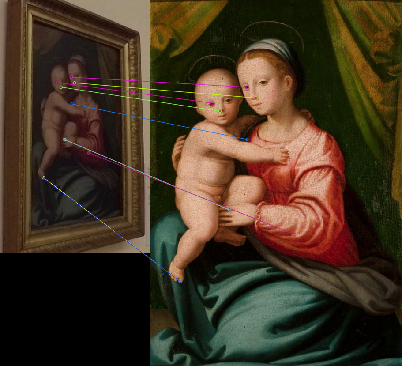
\includegraphics[width=0.4\textwidth]{pictures/painting_retrieval/retrieval}
  \caption{example of painting retrieval}
  \label{fig:retrieval_ex}
\end{figure}

\subsection{Improvements}
To improve the retrieval and to reduce false matches, we used the ratio test described in Lowe's paper \cite{sift}, in order to get the best matches. Given the two best matches (the best match and the second best match) for a keypoint, we define a \(threshold\) and if the ratio between the distance of the two best matches, respectively \(d_1\) and \(d_2\), is above that threshold, \(\frac{d_1}{d_2}>threshold\), we reject that keypoint, considering it equivalent to noise and because the best match is not so different from the second one.

Our goal was to keep the number of paintings correctly found in the database high but at the same time, not decreasing the number of correctly not found paintings that are not in the database. We have chosen \(threshold = 0.6\) because increasing it even by just 0.1, although it decreased the number of positive answer to paintings not listed in the database, this resulted in an increasing number of wrong matches for the paintings in the database. Decreasing the threshold led to an opposite situation and both of the cases didn't meet our goal.

Computing the same keypoints and descriptors for the same paintings in the database has resulted in a slow start, causing the retrieval to wait a couple of seconds or more. Computing the keypoints and descriptors one time and storing them into a file, reduced the retrieval initialization by more than 40\%.
\subsection{Evaluation}
To evaluate the retrieval, we tested it with a sample of 3 random frames per video, with a total of 100 randomly selected videos out of 208. Some of these frames either did not contain any frames or the region of interest of the paintings exceeded the frame size, therefore 100 frames out of the total of 300 were discarded. 266 are the total paintings detected using our trained model and 45 of these were discarded because they were unrecognizable, due to their small size and/or their brightness. 
For the remaining 221 paintings, we manually counted every time we saw a wrong or a right answer. More precisely, we checked if the painting was in the database and the retrieval answer, building the matrix in table \ref{tab:retrieval_eval}.

% Please add the following required packages to your document preamble:
% \usepackage{multirow}
% \usepackage[table,xcdraw]{xcolor}
% If you use beamer only pass "xcolor=table" option, i.e. \documentclass[xcolor=table]{beamer}
\begin{table}
\centering
\begin{tabular}{cccc}
 &
   &
  \multicolumn{2}{c}{\textit{Retrieval answer}} \\ \cline{3-4} 
 &
  \multicolumn{1}{c|}{} &
  \multicolumn{1}{c|}{\textbf{Found}} &
  \multicolumn{1}{c|}{\textbf{\begin{tabular}[c]{@{}c@{}}Wrong or\\ not found\end{tabular}}} \\ \cline{2-4} 
\multicolumn{1}{c|}{} &
  \multicolumn{1}{c|}{\textbf{In DB}} &
  \multicolumn{1}{c|}{58} &
  \multicolumn{1}{c|}{60} \\ \cline{2-4} 
\multicolumn{1}{c|}{\multirow{-3.5}{*}{\rotatebox[origin=c]{90}{\textit{Paintings}}}} &
  \multicolumn{1}{c|}{\textbf{Not in DB}} &
  \multicolumn{1}{c|}{47} &
  \multicolumn{1}{c|}{56} \\ \cline{2-4} 
\end{tabular}
\caption{Painting retrieval evaluation results}
\label{tab:retrieval_eval}
\end{table}
    
The result is that 58 out of 221 paintings were in the database and they were correctly retrieved from it, 56 out of 221 were not in the database but the retrieval correctly gave us a no match found. The remaining paintings are the ones that were wrongly retrieved from the database, 60, and the ones that had not an instance in the database but a wrong match was uncorrectly found.

Accuracy is the measurement used to get information on how good our configuration is: \[ Accuracy = \frac{58+56}{221} \approx 0.52 \]
We think that this result is pretty good, based on the fact that we could increase the real matched paintings, reducing the uncorrectly found paintings that were not actually in the database, adding them manually to it.